\documentclass[twoside]{book}

% Packages required by doxygen
\usepackage{fixltx2e}
\usepackage{calc}
\usepackage{doxygen}
\usepackage[export]{adjustbox} % also loads graphicx
\usepackage{graphicx}
\usepackage[utf8]{inputenc}
\usepackage{makeidx}
\usepackage{multicol}
\usepackage{multirow}
\PassOptionsToPackage{warn}{textcomp}
\usepackage{textcomp}
\usepackage[nointegrals]{wasysym}
\usepackage[table]{xcolor}

% Font selection
\usepackage[T1]{fontenc}
\usepackage[scaled=.90]{helvet}
\usepackage{courier}
\usepackage{amssymb}
\usepackage{sectsty}
\renewcommand{\familydefault}{\sfdefault}
\allsectionsfont{%
  \fontseries{bc}\selectfont%
  \color{darkgray}%
}
\renewcommand{\DoxyLabelFont}{%
  \fontseries{bc}\selectfont%
  \color{darkgray}%
}
\newcommand{\+}{\discretionary{\mbox{\scriptsize$\hookleftarrow$}}{}{}}

% Page & text layout
\usepackage{geometry}
\geometry{%
  a4paper,%
  top=2.5cm,%
  bottom=2.5cm,%
  left=2.5cm,%
  right=2.5cm%
}
\tolerance=750
\hfuzz=15pt
\hbadness=750
\setlength{\emergencystretch}{15pt}
\setlength{\parindent}{0cm}
\setlength{\parskip}{3ex plus 2ex minus 2ex}
\makeatletter
\renewcommand{\paragraph}{%
  \@startsection{paragraph}{4}{0ex}{-1.0ex}{1.0ex}{%
    \normalfont\normalsize\bfseries\SS@parafont%
  }%
}
\renewcommand{\subparagraph}{%
  \@startsection{subparagraph}{5}{0ex}{-1.0ex}{1.0ex}{%
    \normalfont\normalsize\bfseries\SS@subparafont%
  }%
}
\makeatother

% Headers & footers
\usepackage{fancyhdr}
\pagestyle{fancyplain}
\fancyhead[LE]{\fancyplain{}{\bfseries\thepage}}
\fancyhead[CE]{\fancyplain{}{}}
\fancyhead[RE]{\fancyplain{}{\bfseries\leftmark}}
\fancyhead[LO]{\fancyplain{}{\bfseries\rightmark}}
\fancyhead[CO]{\fancyplain{}{}}
\fancyhead[RO]{\fancyplain{}{\bfseries\thepage}}
\fancyfoot[LE]{\fancyplain{}{}}
\fancyfoot[CE]{\fancyplain{}{}}
\fancyfoot[RE]{\fancyplain{}{\bfseries\scriptsize Generated by Doxygen }}
\fancyfoot[LO]{\fancyplain{}{\bfseries\scriptsize Generated by Doxygen }}
\fancyfoot[CO]{\fancyplain{}{}}
\fancyfoot[RO]{\fancyplain{}{}}
\renewcommand{\footrulewidth}{0.4pt}
\renewcommand{\chaptermark}[1]{%
  \markboth{#1}{}%
}
\renewcommand{\sectionmark}[1]{%
  \markright{\thesection\ #1}%
}

% Indices & bibliography
\usepackage{natbib}
\usepackage[titles]{tocloft}
\setcounter{tocdepth}{3}
\setcounter{secnumdepth}{5}
\makeindex

% Hyperlinks (required, but should be loaded last)
\usepackage{ifpdf}
\ifpdf
  \usepackage[pdftex,pagebackref=true]{hyperref}
\else
  \usepackage[ps2pdf,pagebackref=true]{hyperref}
\fi
\hypersetup{%
  colorlinks=true,%
  linkcolor=blue,%
  citecolor=blue,%
  unicode%
}

% Custom commands
\newcommand{\clearemptydoublepage}{%
  \newpage{\pagestyle{empty}\cleardoublepage}%
}

\usepackage{caption}
\captionsetup{labelsep=space,justification=centering,font={bf},singlelinecheck=off,skip=4pt,position=top}

%===== C O N T E N T S =====

\begin{document}

% Titlepage & ToC
\hypersetup{pageanchor=false,
             bookmarksnumbered=true,
             pdfencoding=unicode
            }
\pagenumbering{roman}
\begin{titlepage}
\vspace*{7cm}
\begin{center}%
{\Large My Project }\\
\vspace*{1cm}
{\large Generated by Doxygen 1.8.11}\\
\end{center}
\end{titlepage}
\clearemptydoublepage
\tableofcontents
\clearemptydoublepage
\pagenumbering{arabic}
\hypersetup{pageanchor=true}

%--- Begin generated contents ---
\chapter{File Index}
\section{File List}
Here is a list of all files with brief descriptions\+:\begin{DoxyCompactList}
\item\contentsline{section}{\hyperlink{goal__server_8cpp}{goal\+\_\+server.\+cpp} }{\pageref{goal__server_8cpp}}{}
\item\contentsline{section}{\hyperlink{interface_8cpp}{interface.\+cpp} }{\pageref{interface_8cpp}}{}
\end{DoxyCompactList}

\chapter{File Documentation}
\hypertarget{goal__server_8cpp}{}\section{goal\+\_\+server.\+cpp File Reference}
\label{goal__server_8cpp}\index{goal\+\_\+server.\+cpp@{goal\+\_\+server.\+cpp}}
{\ttfamily \#include \char`\"{}ros/ros.\+h\char`\"{}}\\*
{\ttfamily \#include \char`\"{}final\+\_\+assignment/\+Random\+\_\+\+Goal.\+h\char`\"{}}\\*
Include dependency graph for goal\+\_\+server.\+cpp\+:\nopagebreak
\begin{figure}[H]
\begin{center}
\leavevmode
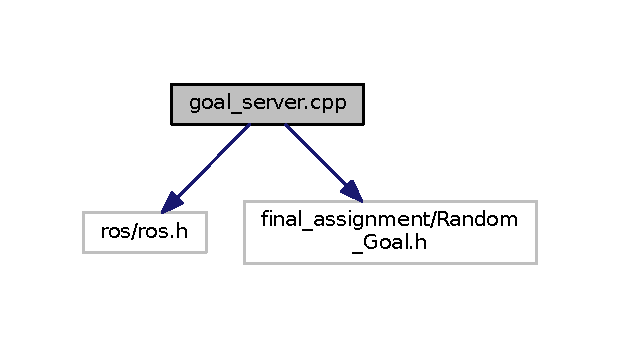
\includegraphics[width=298pt]{goal__server_8cpp__incl}
\end{center}
\end{figure}
\subsection*{Functions}
\begin{DoxyCompactItemize}
\item 
bool \hyperlink{goal__server_8cpp_a1a6af37b07c0c4027195bd55680c687b}{target\+\_\+pos} (final\+\_\+assignment\+::\+Random\+\_\+\+Goal\+::\+Request \&req, final\+\_\+assignment\+::\+Random\+\_\+\+Goal\+::\+Response \&res)
\item 
int \hyperlink{goal__server_8cpp_a3c04138a5bfe5d72780bb7e82a18e627}{main} (int argc, char $\ast$$\ast$argv)
\end{DoxyCompactItemize}


\subsection{Function Documentation}
\index{goal\+\_\+server.\+cpp@{goal\+\_\+server.\+cpp}!main@{main}}
\index{main@{main}!goal\+\_\+server.\+cpp@{goal\+\_\+server.\+cpp}}
\subsubsection[{\texorpdfstring{main(int argc, char $\ast$$\ast$argv)}{main(int argc, char **argv)}}]{\setlength{\rightskip}{0pt plus 5cm}int main (
\begin{DoxyParamCaption}
\item[{int}]{argc, }
\item[{char $\ast$$\ast$}]{argv}
\end{DoxyParamCaption}
)}\hypertarget{goal__server_8cpp_a3c04138a5bfe5d72780bb7e82a18e627}{}\label{goal__server_8cpp_a3c04138a5bfe5d72780bb7e82a18e627}
/\+Main function\+:

/\+Parameters\+:

int argc, char $\ast$$\ast$argv are mandatory for cpp files

/\+Comments about the code\+:

ros\+::init--$>$initialisation of the node position\+\_\+server

ros\+::\+Node\+Handle n --$>$ set-\/up node\+Handle

ros\+::\+Service\+Server service= n.\+advertise\+Service(\char`\"{}robot/random\+\_\+target\char`\"{},target\+\_\+pos); --$>$ define server and specify function call\+Back

ros\+::spin()--$>$ blocks the main thread from exiting until R\+OS invokes a shutdown (for example Ctrl+C) \index{goal\+\_\+server.\+cpp@{goal\+\_\+server.\+cpp}!target\+\_\+pos@{target\+\_\+pos}}
\index{target\+\_\+pos@{target\+\_\+pos}!goal\+\_\+server.\+cpp@{goal\+\_\+server.\+cpp}}
\subsubsection[{\texorpdfstring{target\+\_\+pos(final\+\_\+assignment\+::\+Random\+\_\+\+Goal\+::\+Request \&req, final\+\_\+assignment\+::\+Random\+\_\+\+Goal\+::\+Response \&res)}{target_pos(final_assignment::Random_Goal::Request &req, final_assignment::Random_Goal::Response &res)}}]{\setlength{\rightskip}{0pt plus 5cm}bool target\+\_\+pos (
\begin{DoxyParamCaption}
\item[{final\+\_\+assignment\+::\+Random\+\_\+\+Goal\+::\+Request \&}]{req, }
\item[{final\+\_\+assignment\+::\+Random\+\_\+\+Goal\+::\+Response \&}]{res}
\end{DoxyParamCaption}
)}\hypertarget{goal__server_8cpp_a1a6af37b07c0c4027195bd55680c687b}{}\label{goal__server_8cpp_a1a6af37b07c0c4027195bd55680c687b}
/\+Function call\+Back executed when client calls

/\+Parameters\+: an instance for the request(not used) and an instance for the reply of the srv Random\+\_\+\+Goal.\+srv

/\+Comments about the code\+: \begin{DoxyVerb}        Generate a random number and indices the array of coordinates

        Set the response of the service with the coordinates

        ROS_INFO --> print on screen string between ""\end{DoxyVerb}
 
\hypertarget{interface_8cpp}{}\section{interface.\+cpp File Reference}
\label{interface_8cpp}\index{interface.\+cpp@{interface.\+cpp}}
{\ttfamily \#include \char`\"{}ros/ros.\+h\char`\"{}}\\*
{\ttfamily \#include \char`\"{}stdlib.\+h\char`\"{}}\\*
{\ttfamily \#include \char`\"{}stdio.\+h\char`\"{}}\\*
{\ttfamily \#include \char`\"{}nav\+\_\+msgs/\+Odometry.\+h\char`\"{}}\\*
{\ttfamily \#include \char`\"{}geometry\+\_\+msgs/\+Twist.\+h\char`\"{}}\\*
{\ttfamily \#include \char`\"{}move\+\_\+base\+\_\+msgs/\+Move\+Base\+Action\+Goal.\+h\char`\"{}}\\*
{\ttfamily \#include \char`\"{}final\+\_\+assignment/\+Random\+\_\+\+Goal.\+h\char`\"{}}\\*
{\ttfamily \#include \char`\"{}std\+\_\+srvs/\+Set\+Bool.\+h\char`\"{}}\\*
Include dependency graph for interface.\+cpp\+:\nopagebreak
\begin{figure}[H]
\begin{center}
\leavevmode
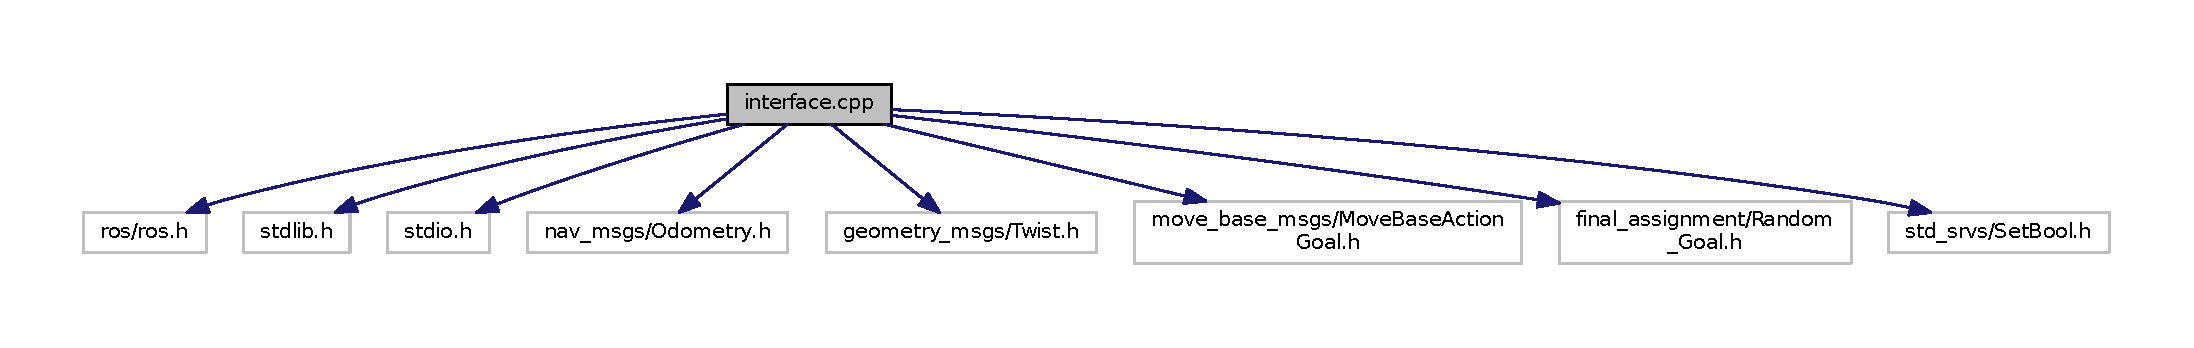
\includegraphics[width=350pt]{interface_8cpp__incl}
\end{center}
\end{figure}
\subsection*{Functions}
\begin{DoxyCompactItemize}
\item 
void \hyperlink{interface_8cpp_aab6e381bffc34921244a29ec0538ba64}{position\+Callback} (const nav\+\_\+msgs\+::\+Odometry\+::\+Const\+Ptr \&msg)
\item 
int \hyperlink{interface_8cpp_a3c04138a5bfe5d72780bb7e82a18e627}{main} (int argc, char $\ast$$\ast$argv)
\end{DoxyCompactItemize}
\subsection*{Variables}
\begin{DoxyCompactItemize}
\item 
ros\+::\+Publisher \hyperlink{interface_8cpp_a350594df3e8f6948c8462edfd41ce086}{pub}
\item 
ros\+::\+Subscriber \hyperlink{interface_8cpp_a24d694a9a8bf73ee31fe92724886a276}{sub}
\item 
move\+\_\+base\+\_\+msgs\+::\+Move\+Base\+Action\+Goal \hyperlink{interface_8cpp_a3c603a803d713e1425a427fe6cff6b62}{target}
\item 
float \hyperlink{interface_8cpp_a103d17f7ae810b61a0196086a9642477}{x\+\_\+pos}
\item 
float \hyperlink{interface_8cpp_a17c98f6e8cadb148806771b487612871}{y\+\_\+pos}
\item 
final\+\_\+assignment\+::\+Random\+\_\+\+Goal \hyperlink{interface_8cpp_a543008507956de814cfdd70448a5c211}{random\+\_\+target}
\item 
std\+\_\+srvs\+::\+Set\+Bool \hyperlink{interface_8cpp_a47e3eaec83c24b79b71e245205fdb431}{wall\+\_\+follow}
\end{DoxyCompactItemize}


\subsection{Function Documentation}
\index{interface.\+cpp@{interface.\+cpp}!main@{main}}
\index{main@{main}!interface.\+cpp@{interface.\+cpp}}
\subsubsection[{\texorpdfstring{main(int argc, char $\ast$$\ast$argv)}{main(int argc, char **argv)}}]{\setlength{\rightskip}{0pt plus 5cm}int main (
\begin{DoxyParamCaption}
\item[{int}]{argc, }
\item[{char $\ast$$\ast$}]{argv}
\end{DoxyParamCaption}
)}\hypertarget{interface_8cpp_a3c04138a5bfe5d72780bb7e82a18e627}{}\label{interface_8cpp_a3c04138a5bfe5d72780bb7e82a18e627}
M\+A\+IN F\+U\+N\+C\+T\+I\+ON

/\+Parameters\+: int argc, char $\ast$$\ast$argv are mandatory for cpp files

/\+Comments about the code\+:

Declare a Rate of 1 Hz for call periodically ros\+::spin\+Once\+:\+:

pub=n.\+advertise$<$move\+\_\+base\+\_\+msgs\+::\+Move\+Base\+Action\+Goal$>$(\char`\"{}move\+\_\+base/goal\char`\"{},1000) --$>$ Define a Publisher on topic \char`\"{}move\+\_\+base/goal\char`\"{}

sub=n.\+subscribe(\char`\"{}/odom\char`\"{},1000,position\+Callback) --$>$ Define a Subscriber that publish on topic /odom the position

x\+\_\+coordintes and y\+\_\+coordinates are the two array of possibles coordinates

Declare client1 of type final\+\_\+assignment\+::\+Random\+\_\+\+Goal that will do the request on robot/random\+\_\+target service

Declare client2 of type std\+\_\+srvs\+::\+Set\+Bool that will do the request on wall\+\_\+follower\+\_\+switch service

if(command==1) \begin{DoxyVerb}with client1 call pull a random_target and publish on move_base
\end{DoxyVerb}


if(command==2) \begin{DoxyVerb}user choose one of possible coordinates and publish it on move_base
\end{DoxyVerb}


if(command==3) \begin{DoxyVerb}set the argument of the request=true and with client2 call the wall_follow service
\end{DoxyVerb}


if(command==4) \begin{DoxyVerb}set the argument of the request=false and publish on move_base the current position to stop the Robot\end{DoxyVerb}
 \index{interface.\+cpp@{interface.\+cpp}!position\+Callback@{position\+Callback}}
\index{position\+Callback@{position\+Callback}!interface.\+cpp@{interface.\+cpp}}
\subsubsection[{\texorpdfstring{position\+Callback(const nav\+\_\+msgs\+::\+Odometry\+::\+Const\+Ptr \&msg)}{positionCallback(const nav_msgs::Odometry::ConstPtr &msg)}}]{\setlength{\rightskip}{0pt plus 5cm}void position\+Callback (
\begin{DoxyParamCaption}
\item[{const nav\+\_\+msgs\+::\+Odometry\+::\+Const\+Ptr \&}]{msg}
\end{DoxyParamCaption}
)}\hypertarget{interface_8cpp_aab6e381bffc34921244a29ec0538ba64}{}\label{interface_8cpp_aab6e381bffc34921244a29ec0538ba64}
/\+Function position\+Call\+Back called when subscriber receives the position

/-\/\+Parameter\+:

msg\+: declared as constant pointer of topic Odom (to establish the position of the robot)

/\+The funcion save on global variables the position of the Robot so i can reuse it on main 

\subsection{Variable Documentation}
\index{interface.\+cpp@{interface.\+cpp}!pub@{pub}}
\index{pub@{pub}!interface.\+cpp@{interface.\+cpp}}
\subsubsection[{\texorpdfstring{pub}{pub}}]{\setlength{\rightskip}{0pt plus 5cm}ros\+::\+Publisher pub}\hypertarget{interface_8cpp_a350594df3e8f6948c8462edfd41ce086}{}\label{interface_8cpp_a350594df3e8f6948c8462edfd41ce086}
Define Publisher that will publish velocity of robot on topic move\+\_\+base/goal \index{interface.\+cpp@{interface.\+cpp}!random\+\_\+target@{random\+\_\+target}}
\index{random\+\_\+target@{random\+\_\+target}!interface.\+cpp@{interface.\+cpp}}
\subsubsection[{\texorpdfstring{random\+\_\+target}{random_target}}]{\setlength{\rightskip}{0pt plus 5cm}final\+\_\+assignment\+::\+Random\+\_\+\+Goal random\+\_\+target}\hypertarget{interface_8cpp_a543008507956de814cfdd70448a5c211}{}\label{interface_8cpp_a543008507956de814cfdd70448a5c211}
random\+\_\+target a global instance of service Random\+\_\+\+Goal \index{interface.\+cpp@{interface.\+cpp}!sub@{sub}}
\index{sub@{sub}!interface.\+cpp@{interface.\+cpp}}
\subsubsection[{\texorpdfstring{sub}{sub}}]{\setlength{\rightskip}{0pt plus 5cm}ros\+::\+Subscriber sub}\hypertarget{interface_8cpp_a24d694a9a8bf73ee31fe92724886a276}{}\label{interface_8cpp_a24d694a9a8bf73ee31fe92724886a276}
Define the subscriber that will publish on topic /odom \index{interface.\+cpp@{interface.\+cpp}!target@{target}}
\index{target@{target}!interface.\+cpp@{interface.\+cpp}}
\subsubsection[{\texorpdfstring{target}{target}}]{\setlength{\rightskip}{0pt plus 5cm}move\+\_\+base\+\_\+msgs\+::\+Move\+Base\+Action\+Goal target}\hypertarget{interface_8cpp_a3c603a803d713e1425a427fe6cff6b62}{}\label{interface_8cpp_a3c603a803d713e1425a427fe6cff6b62}
Instance target of topic move\+\_\+base\+\_\+msgs\+::\+Move\+Base\+Action\+Goal

This will be able to set the coordinates of the goal and Robot will reach it \index{interface.\+cpp@{interface.\+cpp}!wall\+\_\+follow@{wall\+\_\+follow}}
\index{wall\+\_\+follow@{wall\+\_\+follow}!interface.\+cpp@{interface.\+cpp}}
\subsubsection[{\texorpdfstring{wall\+\_\+follow}{wall_follow}}]{\setlength{\rightskip}{0pt plus 5cm}std\+\_\+srvs\+::\+Set\+Bool wall\+\_\+follow}\hypertarget{interface_8cpp_a47e3eaec83c24b79b71e245205fdb431}{}\label{interface_8cpp_a47e3eaec83c24b79b71e245205fdb431}
wall\+\_\+follow a global instance of std\+\_\+srvs that will call wall\+\_\+follow service \index{interface.\+cpp@{interface.\+cpp}!x\+\_\+pos@{x\+\_\+pos}}
\index{x\+\_\+pos@{x\+\_\+pos}!interface.\+cpp@{interface.\+cpp}}
\subsubsection[{\texorpdfstring{x\+\_\+pos}{x_pos}}]{\setlength{\rightskip}{0pt plus 5cm}float x\+\_\+pos}\hypertarget{interface_8cpp_a103d17f7ae810b61a0196086a9642477}{}\label{interface_8cpp_a103d17f7ae810b61a0196086a9642477}
Define global two float variables for the instantaneous position of the robot \index{interface.\+cpp@{interface.\+cpp}!y\+\_\+pos@{y\+\_\+pos}}
\index{y\+\_\+pos@{y\+\_\+pos}!interface.\+cpp@{interface.\+cpp}}
\subsubsection[{\texorpdfstring{y\+\_\+pos}{y_pos}}]{\setlength{\rightskip}{0pt plus 5cm}float y\+\_\+pos}\hypertarget{interface_8cpp_a17c98f6e8cadb148806771b487612871}{}\label{interface_8cpp_a17c98f6e8cadb148806771b487612871}

%--- End generated contents ---

% Index
\backmatter
\newpage
\phantomsection
\clearemptydoublepage
\addcontentsline{toc}{chapter}{Index}
\printindex

\end{document}
